% !TeX spellcheck = german
\documentclass[9pt,a4paper]{report}
\usepackage[T1,EU1]{fontenc}    
\usepackage[utf8]{inputenc} 
\usepackage[ngerman]{babel}

\usepackage[bookmarks=true, pdfborder={0 0 0}]{hyperref}
\usepackage[ngerman]{cleveref}

\hypersetup{
	colorlinks=true,      % Rahmen entfernen und Text einfärben
	linkcolor=blue,       % Farbe für interne Verweise (Tabellen, Kapitel, etc.)
	urlcolor=blue,        % Farbe für Web-Adressen
	citecolor=green!60!black % Farbe für Zitate (Dunkelgrün)
}


\usepackage{graphicx}

% --- CODE SETUP

\usepackage{listings}
\usepackage{xcolor}

\lstset{inputpath={{../02_Software/}}}

% Define colors for the code
\definecolor{codegreen}{rgb}{0,0.6,0}
\definecolor{codegray}{rgb}{0.5,0.5,0.5}
\definecolor{codepurple}{rgb}{0.58,0,0.82}
\definecolor{backcolour}{rgb}{0.95,0.95,0.92}

% Setup the style
\lstset{
	language=Python,
	backgroundcolor=\color{backcolour},   
	commentstyle=\color{codegreen},
	keywordstyle=\color{magenta},
	numberstyle=\tiny\color{codegray},
	stringstyle=\color{codepurple},
	basicstyle=\ttfamily\small,
	breakatwhitespace=false,         
	breaklines=true,                 
	captionpos=b,                    
	keepspaces=true,                 
	numbers=left,                    % Line numbers on the left
	numbersep=5pt,                  
	showspaces=false,                
	showstringspaces=false,
	showtabs=false,                  
	tabsize=2
}

\title{ESP32 Wetter Station Teil 1}
\author{Anthony Timmel}

\begin{document}
	\maketitle
	\tableofcontents
	\cleardoublepage
	\part{Einführung}
	In dem ersten Teil dieser Dokumentation beschäftigen wir uns mit dem ersten Teil der Aufgabe aus dem Unterricht LF7. In den nächsten Seiten wird Ihnen das Projekt \textit{Wetterstation ESP32} im ersten Teil schriftlich vorgestellt. Dabei werden wir uns zuerst die benötigten Hardwarekomponenten anschauen, danach folgt die Verkabelung dieser Komponenten mit dem \textit{ESP32} \& am Ende schauen wir uns die Umsetzung in dem Quelltext an.
	
	\chapter{Pinarten des ESP32}
	In diesem Projekt verwenden wir mehrere unterschiedliche so genannte \textbf{Pins}. Dies sind spezielle Arten von Anschlüssen, die natürlich auch unterschiedlichen Zwecken dienen. Hier werden wir auf eine Handvoll eingehen, die auch tatsächlich im Projekt genutzt werden. Dabei unterscheiden sich diese immer in der Art \& Weise, wie Daten von der Komponente \& dem \textit{ESP32} übertragen werden.
	\section{GPIO}
	GPIO steht für \textbf{General Purpose Input/Output}. Dabei kann dieser entweder ein Eingangs- oder Ausgangssignal repräsentieren. Es wird dazu genutzt, um mit weiteren einfachen Komponenten zu kommunizieren oder Steuern.
	
	\begin{figure}[h]
		\centering
		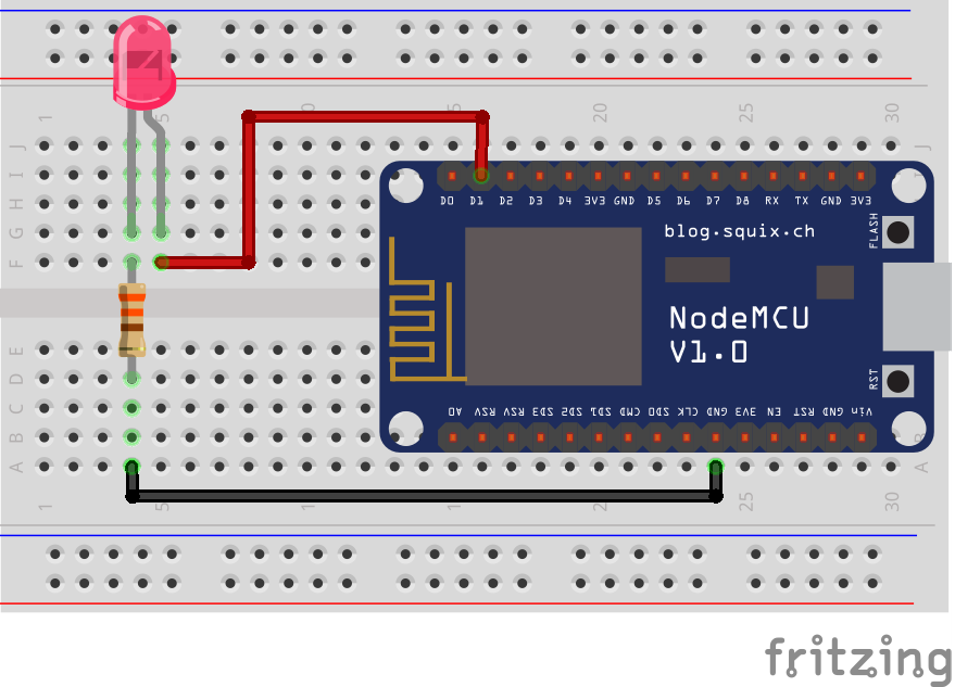
\includegraphics[width=0.7\linewidth]{assets/gpio-pin-theory}
		\caption[GPIO Aufbau]{Dieses Bild zeigt den Aufbau von einem GPIO Port mit einer LED, die an den ESP32 angeschlossen ist.}
		\label{fig:gpio-pin-theory2}
	\end{figure}
	
	\section{I2C}
	I2C oder auch \textbf{Inter-Integrated-Circuit} ist ein serieller Kommunikationsbus, der 2 spezielle GPIO Pins benötigt \textbf{SDA}(Serial Data Line) \& \textbf{SCL}(Serial Clock Line). Dabei wird \textit{I2C} benötigt, um Daten schnell \& in großer Form zu übertragen, sowie die Uhrzeit synchron über Komponenten hinweg zu halten.
	\begin{figure}[h]
		\centering
		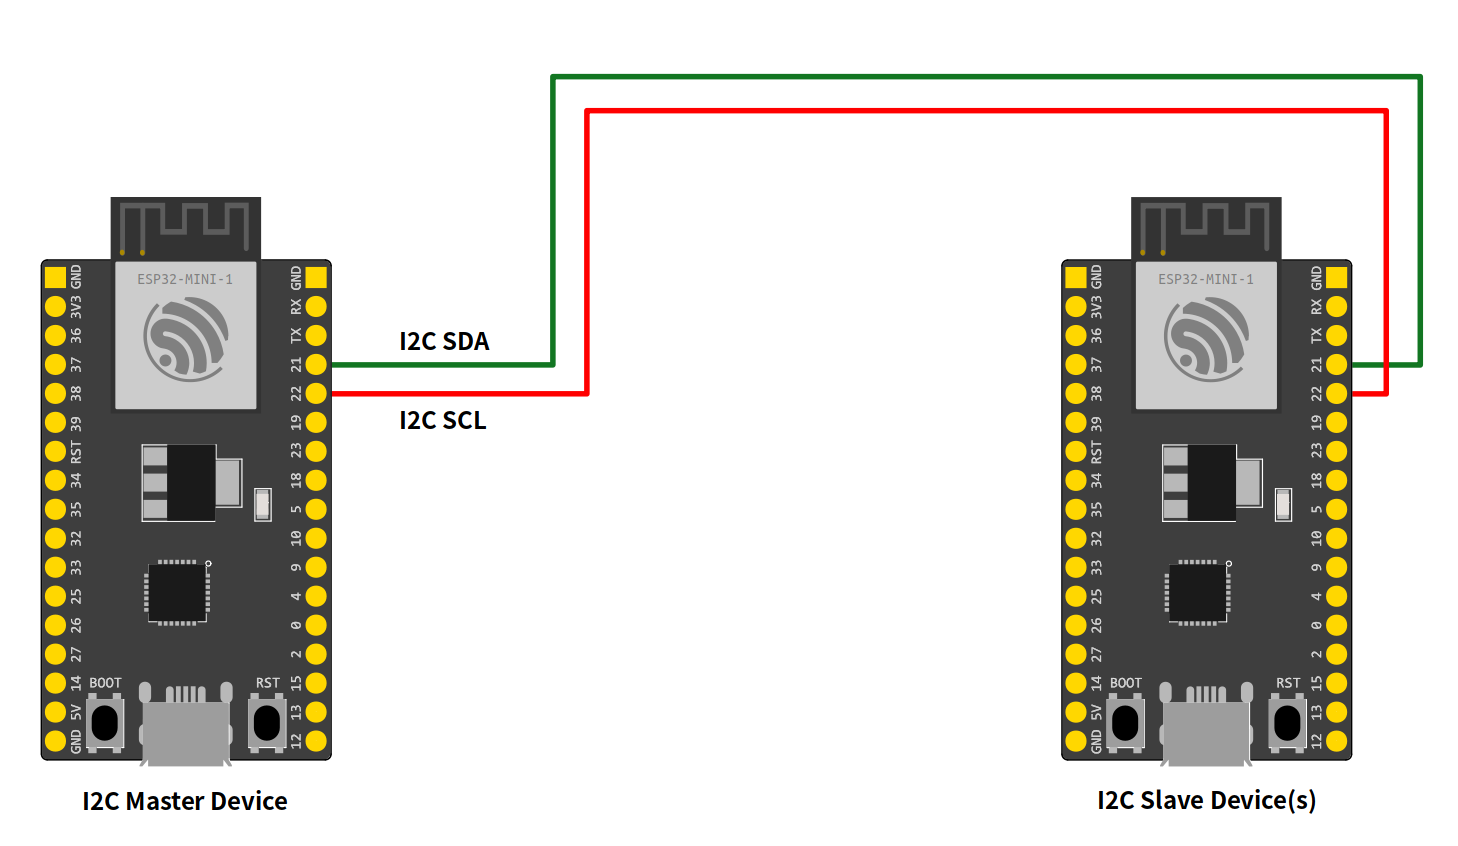
\includegraphics[width=0.7\linewidth]{assets/i2c-schema}
		\caption[I2C Aufbau]{Dieses Bild zeigt den Aufbau von I2C. In diesem Bild sind 2 \textit{ESP32} miteinander Verbunden, dabei können sie Daten schnell \& einfach Übertragen. Diese Verbindung benötigt jedoch einen Verantwortlichen \textit{auch Master genannt}. Jedes weitere Bauteil in dieser Verbindung ist ein Slave, dieser hört priorisiert auf die Anweisungen vom Master, kann jedoch, je nach Einstellungen, auch die gleichen Operationen wie der Master.}
		\label{fig:i2c-schema}
	\end{figure}
	
	\section{SPI}
	SPI steht für \textbf{Serial Peripheral Interface} und ist ein synchrones serielles Datenprotokoll, das von einem Mikrocontroller (Controller oder auch Master genannt) zur Kommunikation mit einem oder mehreren Peripheriegeräten (auch Slaves genant) verwendet wird. Beispielsweise kommuniziert der ESP32-Board mit einem Sensor, der SPI unterstützt, oder mit einem anderen Mikrocontroller.
	\begin{figure}[h]
		\centering
		\caption{SPI Aufbau}
		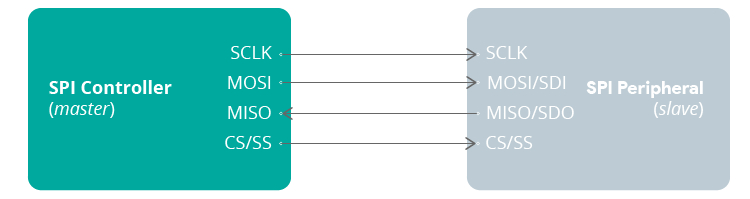
\includegraphics[height=0.5\textheight, width=\textwidth, keepaspectratio]{assets/SPI-communication.jpg}
	\end{figure}
	
	\chapter{Der Aufbau des ESP32 auf dem Board}
	\section{Versorgungs- \& Datenplan des ESP32}
	\begin{figure}[h]
		\centering
		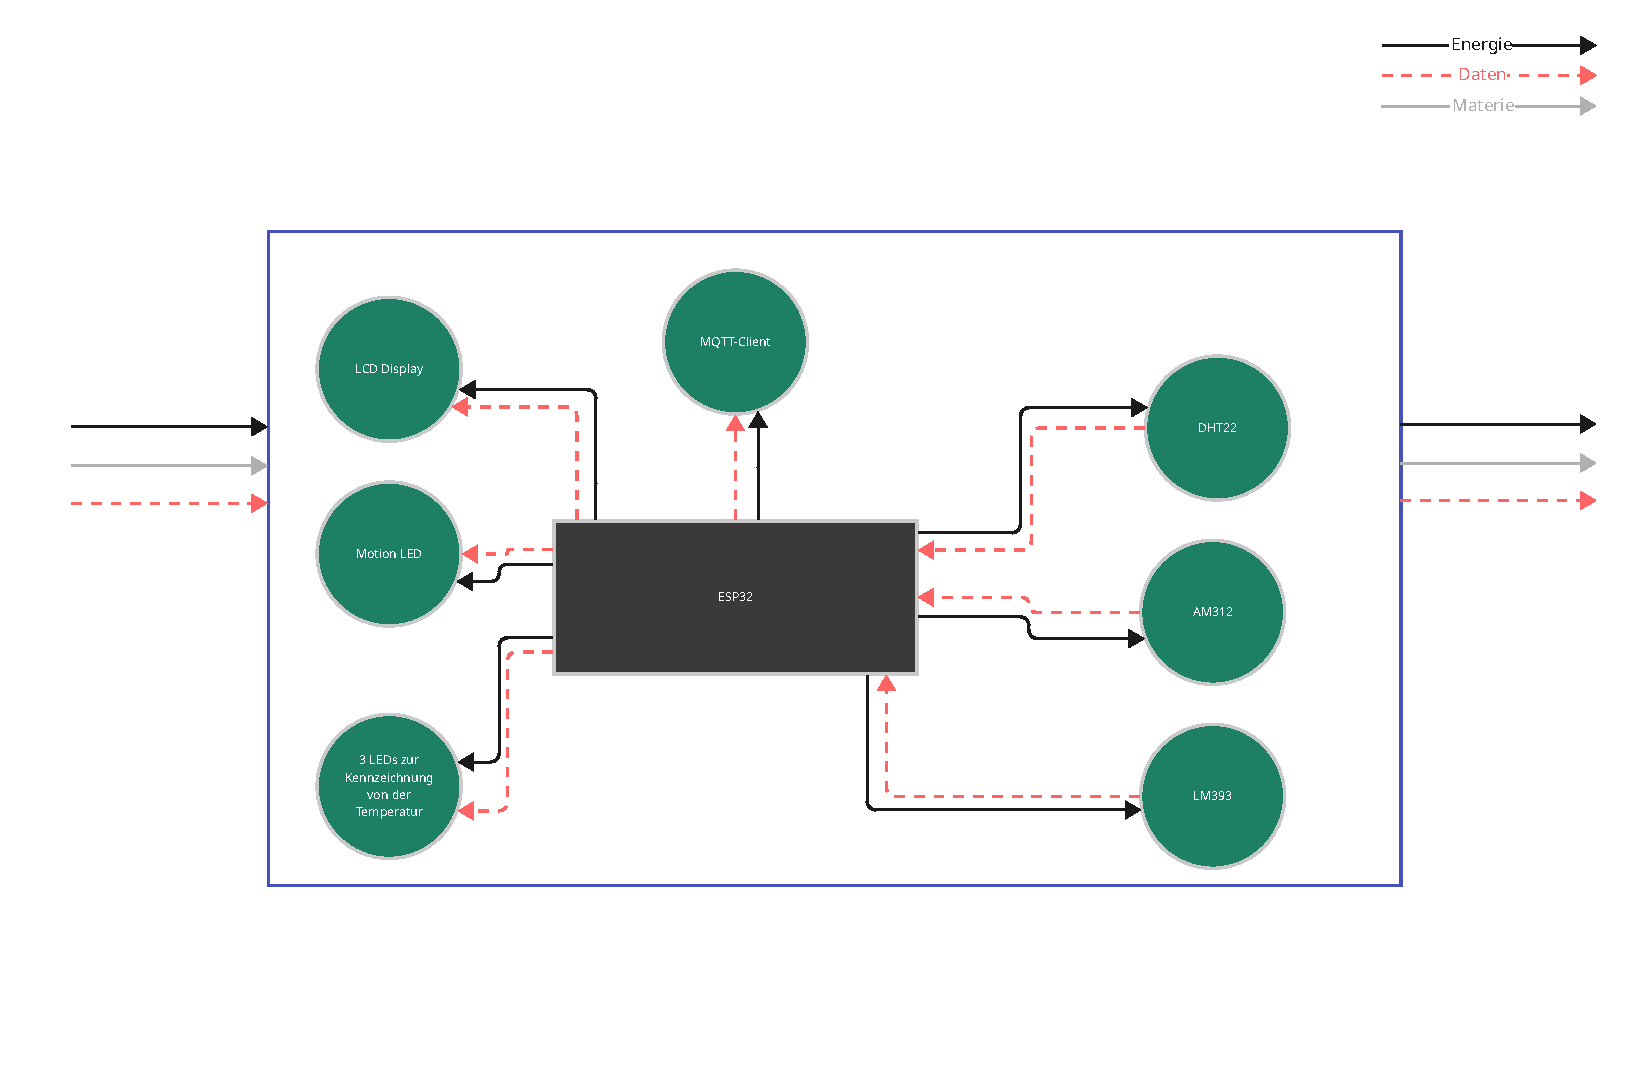
\includegraphics[width=0.7\linewidth]{assets/ESP32_Structure}
		\caption[Aufbaue des ESP32]{Aufbau es ESP32 auf dem Board. Diese Abbildung beinhaltet bereits Module, die nicht in dieser Dokumentation erklärt wurden. Diese Abbildung wurde dennoch zur Vollständigkeit nicht abgeändert. In der Dokumentation Teil 2, befindet sich dann die fehlenden Modulen}
		\label{fig:esp32structure}
	\end{figure}
	\newpage
	\section{Draufsicht auf den ESP32 in Betrieb}
	\begin{figure}[h]
		\centering
		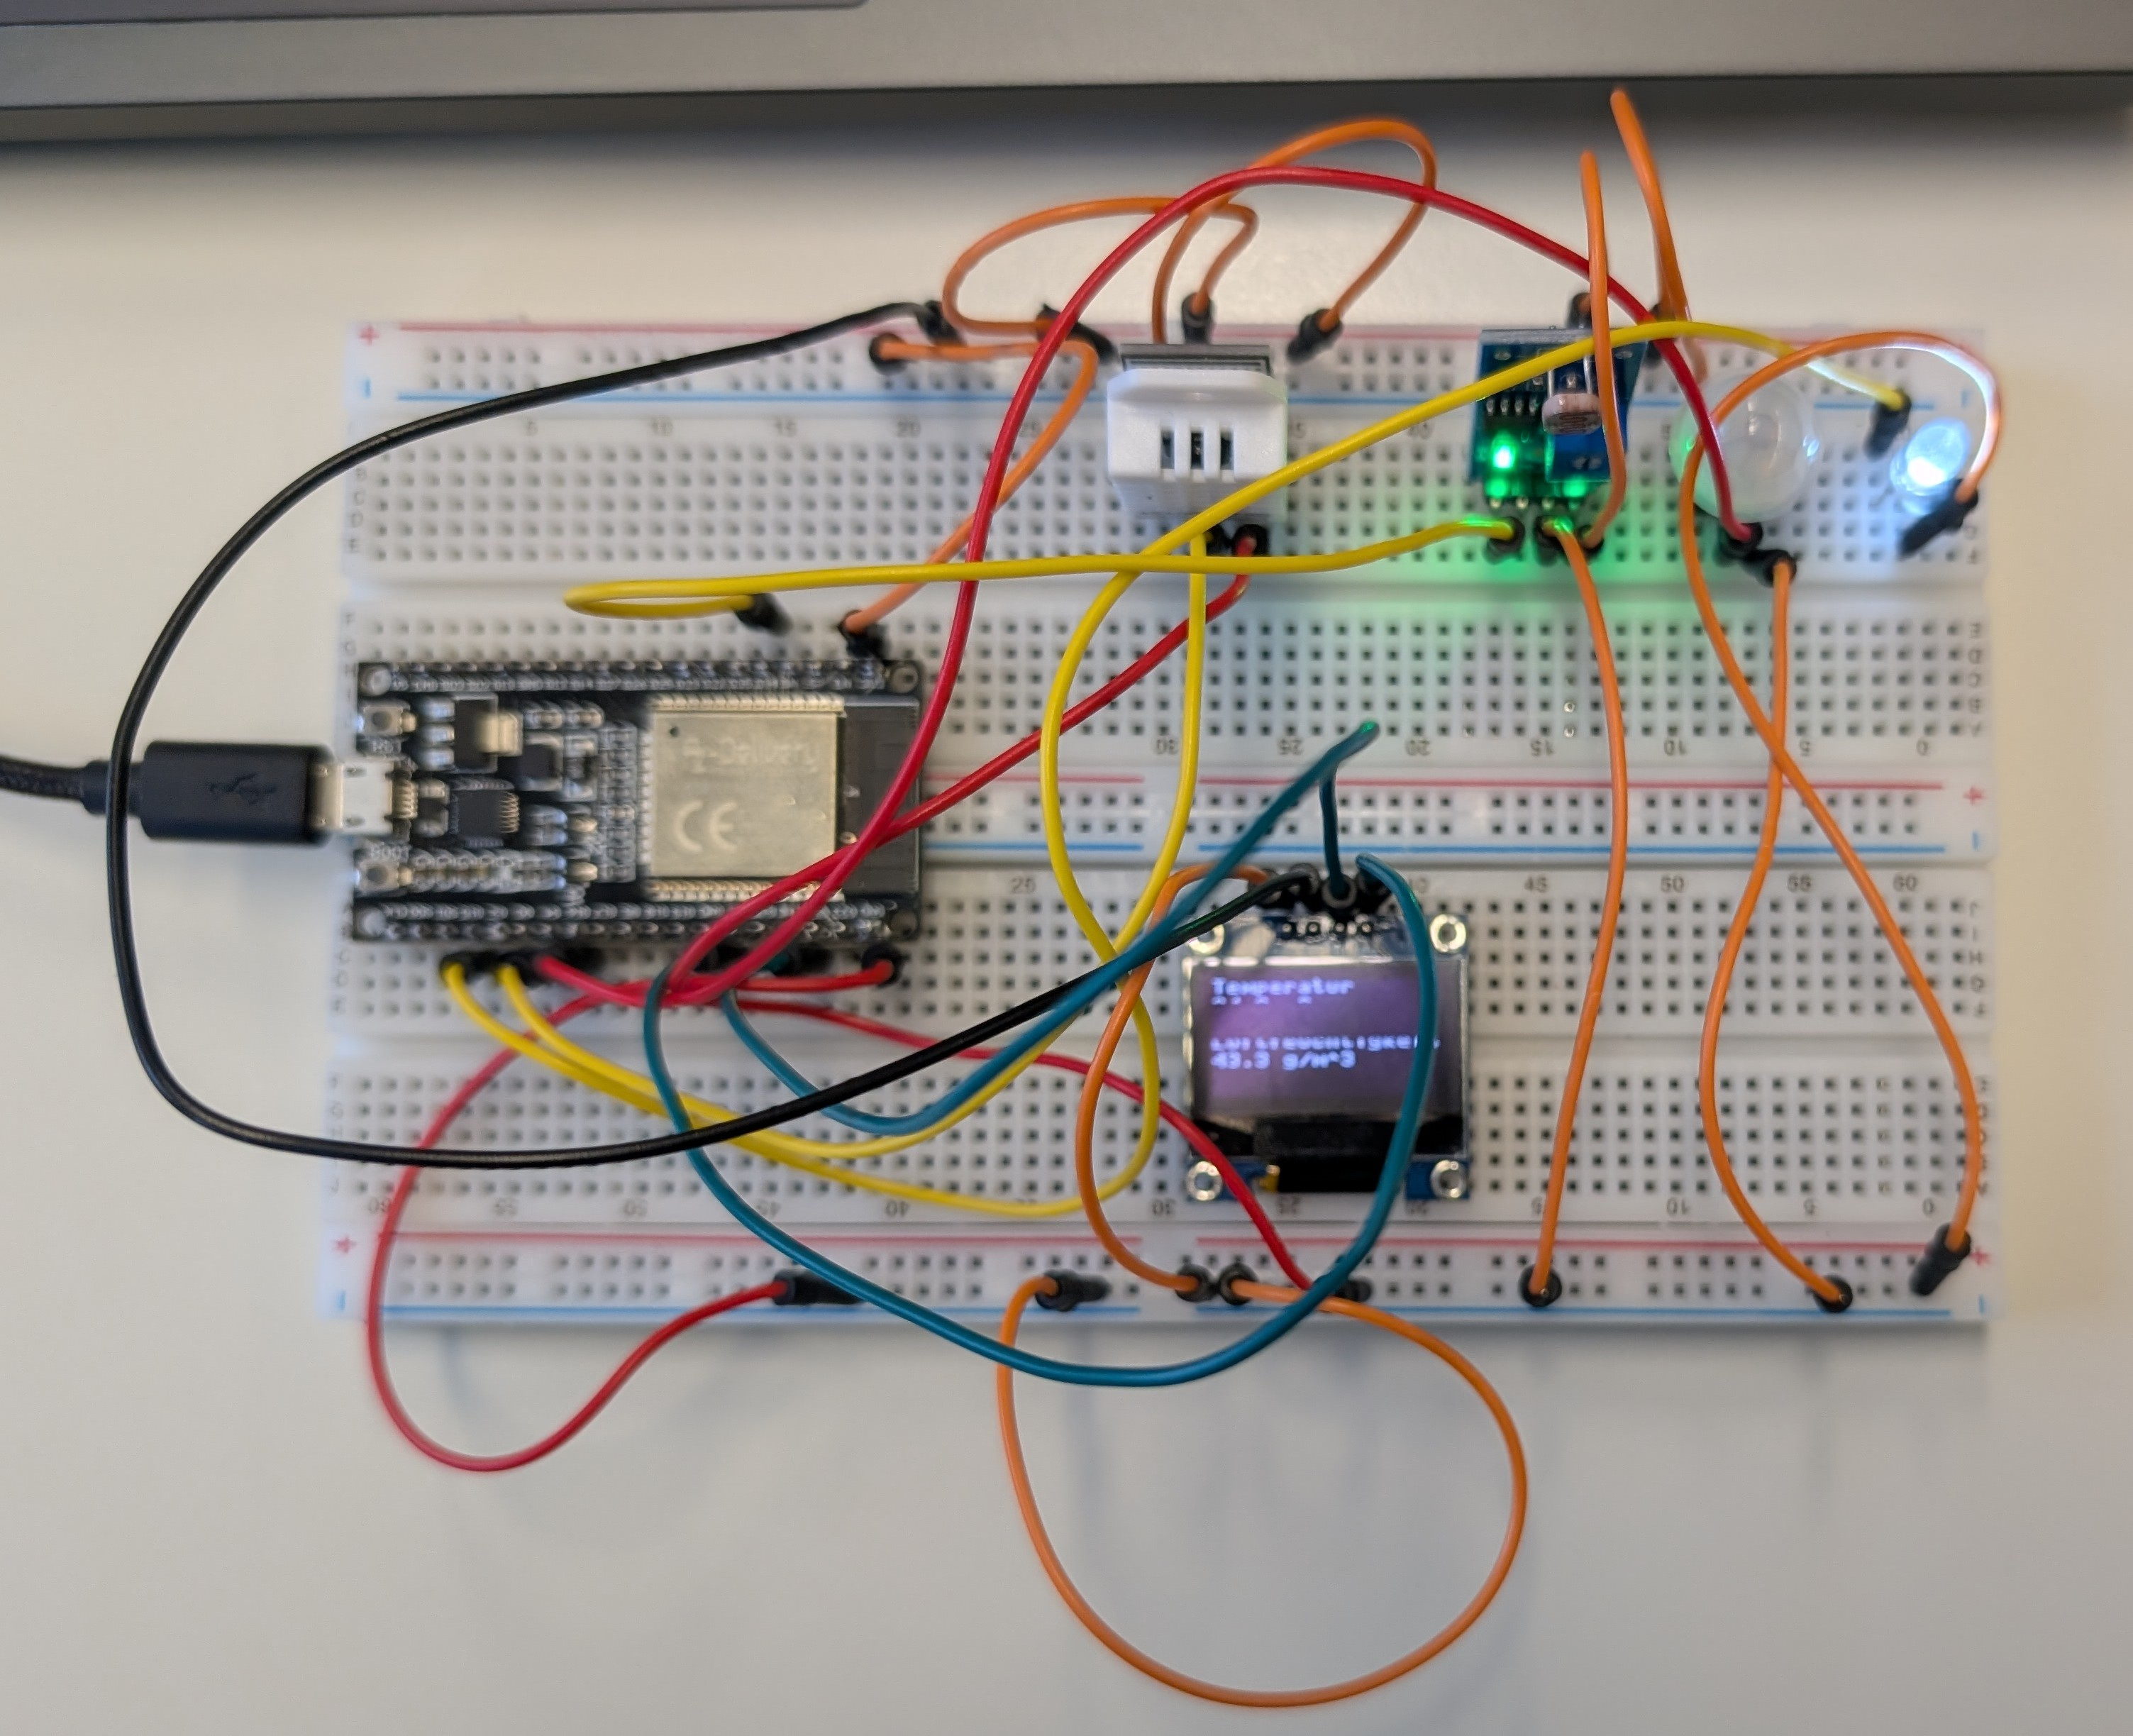
\includegraphics[width=0.7\linewidth]{assets/esp32_top-view}
		\caption[Draufsicht auf die Bauteile des ESP32]{In dieser Draufsicht sehen Sie das fertig gebaute Produkt aus dem Projekt Teil 1. Die Bauteile sind hier bereits mit dem ESP32 verbunden \& der benötigte Quelltext ist in einem kompletten funktionalen Zustand.}
		\label{fig:esp32top-view}
	\end{figure}
	\newpage
		\section{Nebenansicht auf den ESP32 in Betrieb}
	\begin{figure}[h]
		\centering
		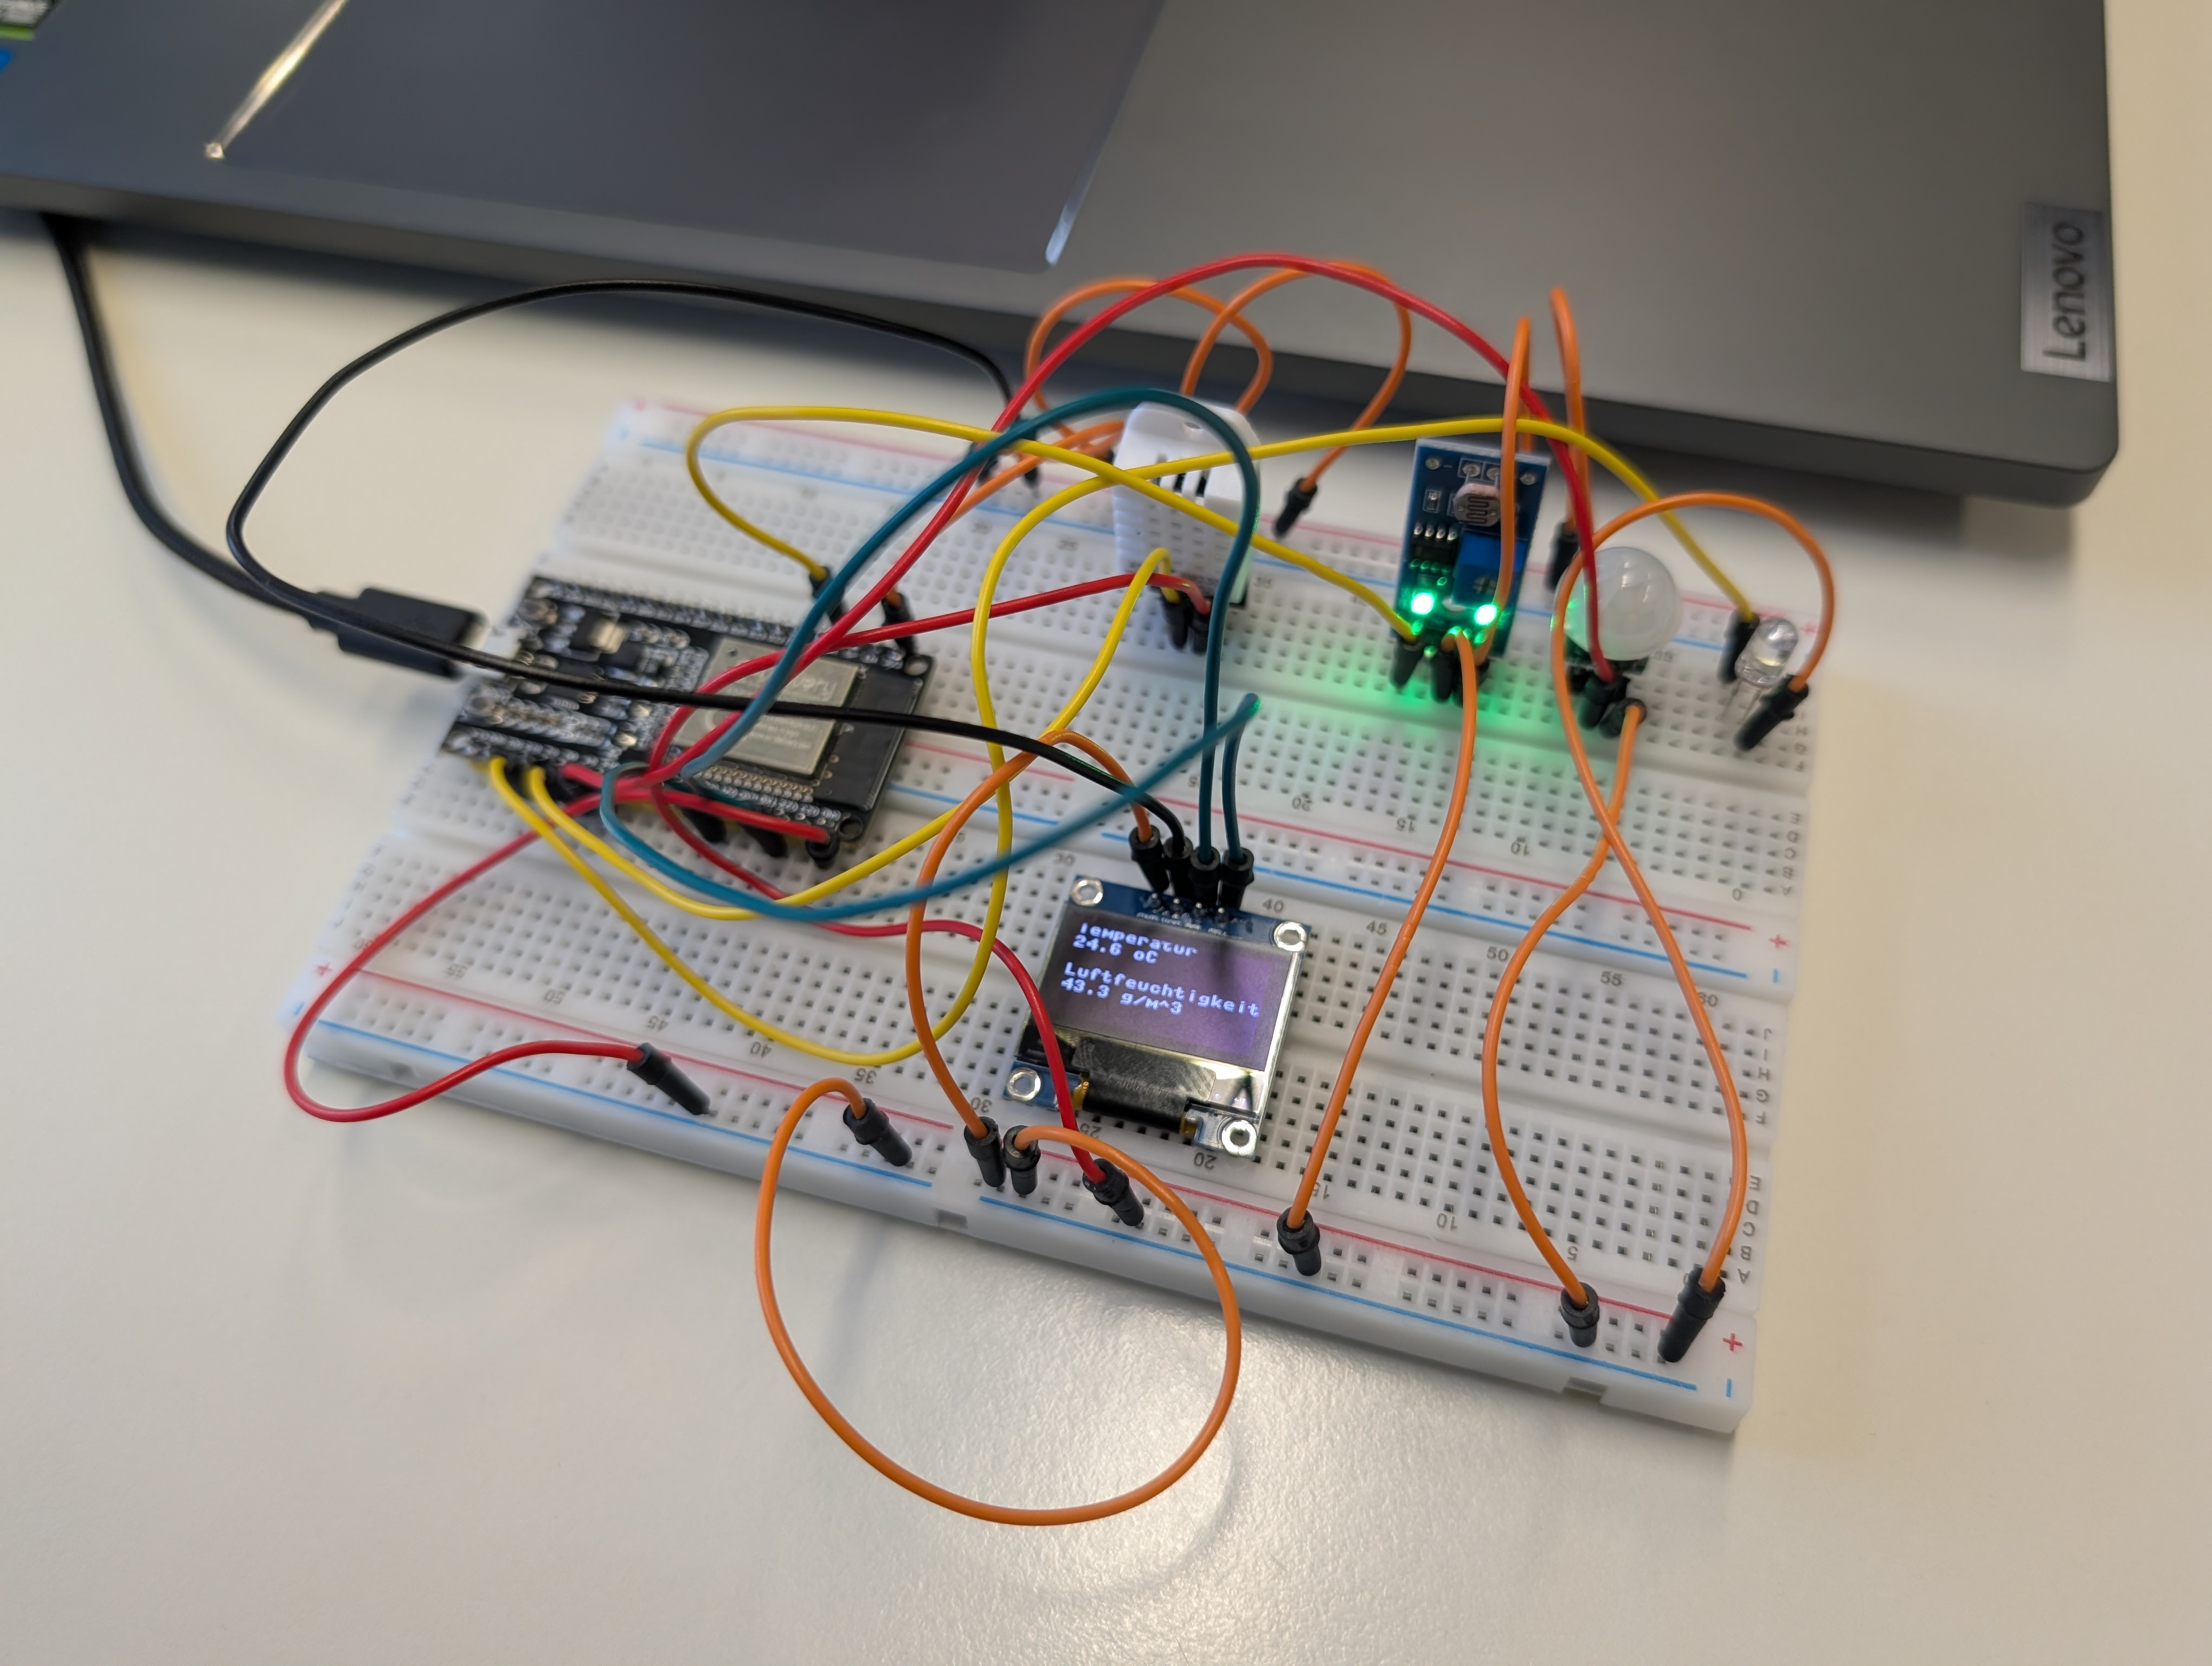
\includegraphics[width=0.7\linewidth]{assets/esp32_side-view}
		\caption[Nebenansicht auf den ESP32]{In dieser Nebenansicht sehen Sie das fertig gebaute Produkt aus dem Projekt Teil 1. Die Bauteile sind hier bereits mit dem ESP32 verbunden \& der benötigte Quelltext ist in einem kompletten funktionalen Zustand.}
		\label{fig:esp32side-view}
	\end{figure}
	
	\section{Programmierung des ESP32}
	Damit der ESP32 \& die anderen Komponenten miteinander Kommunizieren kann sowie die Weitergabe der Daten an externe Dienste, müssen diese Funktionen zum Teil manuell als Programmiercode geschrieben werden. Hierbei benutzten wir eine einfachere Variante, indem wir Python als Programmiersprache verwenden. Zusammen mit der Erweiterung für Microcontroller namens MicroPython können wir den ESP32 in einfachen Schritten anleiten, bestimmte Aufgaben zu erledigen.
	
	\newpage
	\subsection{Klassen}
	Bestimmte Klassen werden in den Code-Snippets immer wieder vorkommen. Dabei handelt es sich um wesentliche Grundfunktionen von Micropython oder Python an sich.
	Klassen die nicht in dieser Auflistung sind, werden in der Aufgabe, in der diese das erste mal genutzt werden, erklärt.
	
	\subsubsection{Pin}
	Die \texttt{Pin} Klasse wird in Micropython verwendet, um eine Schnittstelle zwischen dem ESP32 \& der Komponente auf dem Steckbrett zu deklarieren.
	Eine Deklaration eines Pins sieht wie folgend aus:
	\begin{lstlisting}
	PIN_VALUE = 1
	PIN_IO = Pin.OUT
	PIN_DRIVE = Pin.DRIVE_0
	pin = Pin(PIN_VALUE, PIN_IO, drive=PIN_DRIVE)
	\end{lstlisting}
	\begin{enumerate}
		\item \texttt{PIN\_VALUE} => GPIO Nummer des Pins. Zusehen ist diese auf der Abbildung \ref{fig:esp32-pins}
		\item \texttt{PIN\_IO} => I/O Richtung des Pins. Hierbei wählt man zwischen \texttt{Pin.IN} (\textit{Eingehend}) oder \texttt{Pin.OUT} (\textit{Ausgehend}). Der Pin agiert dann ausschließlich in diese Richtung.
		\item \texttt{PIN\_DRIVE} => Die Ausgabe von der Stromstärke in 4 verschiedenen Stufen.  (\textbf{Optional})
	\end{enumerate}
	
	Die offizielle Dokumentation befindet sich auf der \hyperref{https://docs.micropython.org/en/latest/esp32/quickref.html#pins-and-gpio}{micropython}{MicroPython Pin \& GPIO}{MicroPython} Seite. Dort befindet sich eine ausführliche Erklärung der verschiedenen Variablen für die Erstellung einer Instanz der \texttt{Pin} Klasse.
	
	\begin{figure}[h]
		\centering
		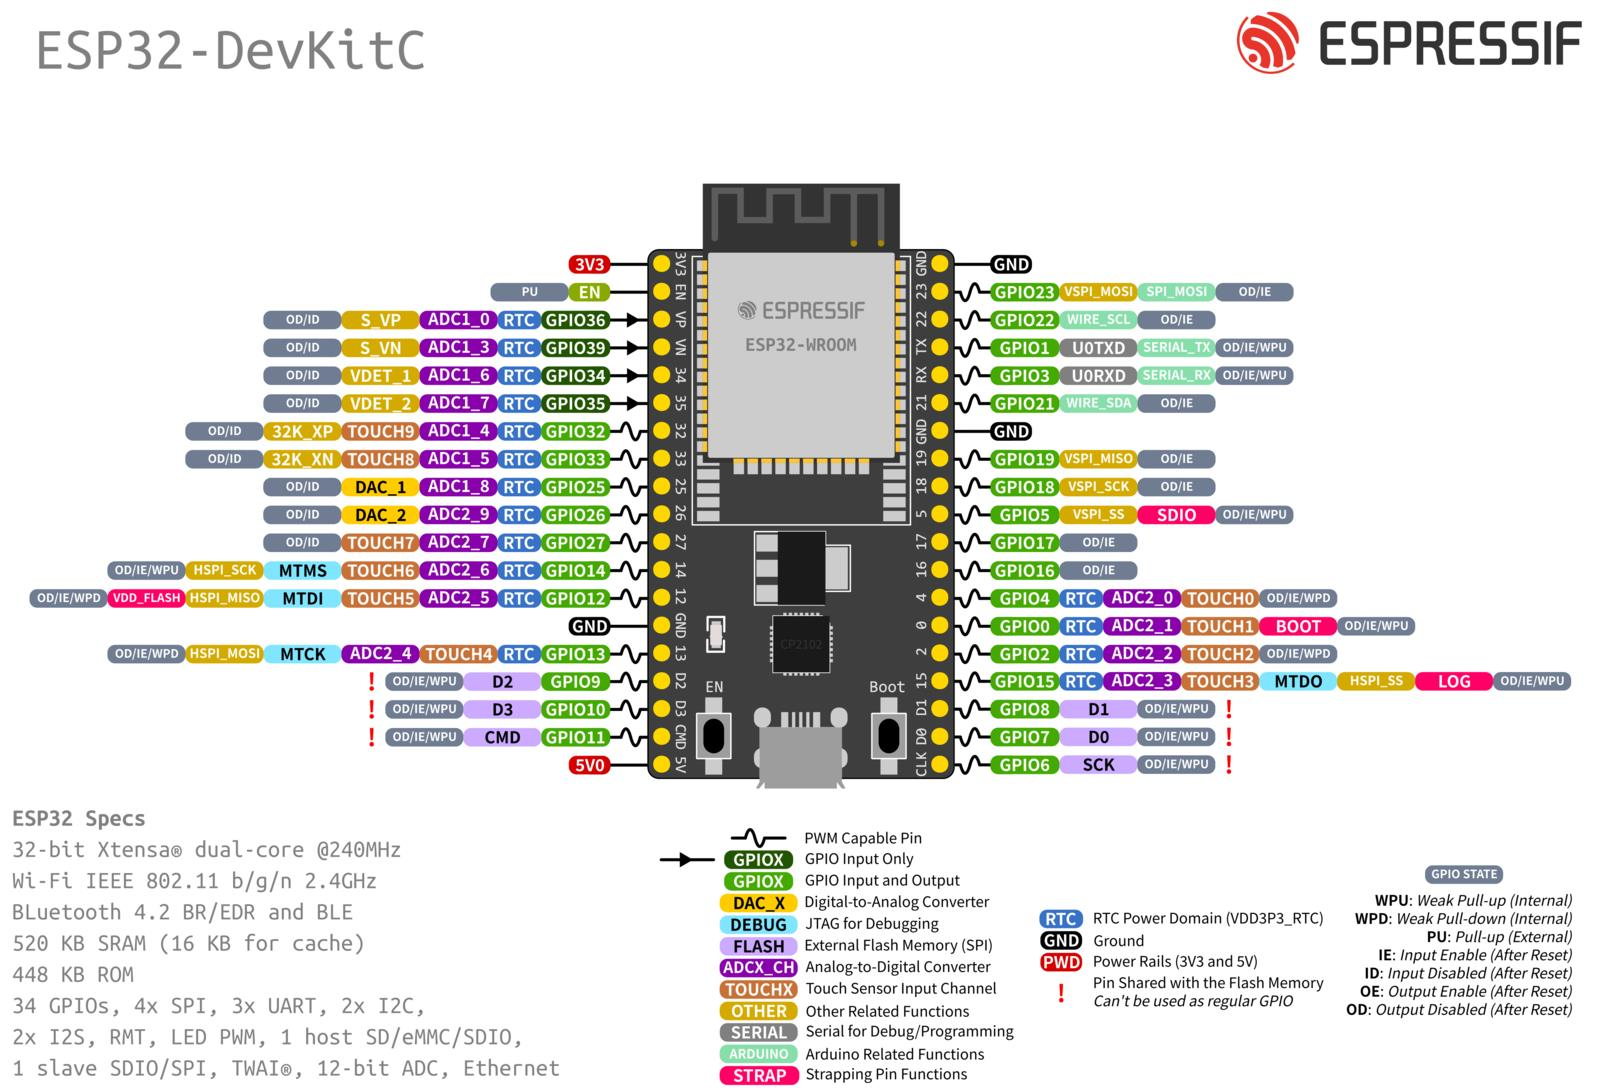
\includegraphics[width=\linewidth]{assets/esp32-pins}
		\caption[Pinverteilung an dem ESP32]{In dieser Abbildung sehen Sie die Verteilen der Pins auf dem ESP32. In den folgenden Tabellen innerhalb der Bauelemente Sektion, werden Referenzen zu dieser Übersicht gemacht.}
		\label{fig:esp32-pins}
	\end{figure}
	
	\newpage
	\subsection{Funktionen}
	In unserer Anwendung benutzen wir ebenfalls vordefinierte Funktionen, aus Micropython oder Python an sich.
	
	\subsubsection{sleep}
	Die \texttt{sleep} Funktion ermöglicht uns, den Prozess für eine bestimmte Zeit anzuhalten.
	\begin{lstlisting}
	sleep(1)
	\end{lstlisting}
	Hierbei pausieren wir den Prozess für 1 Sekunde.
	
	\subsubsection{print}
	Die \texttt{print} Funktion gibt uns Text in der Befehlszeile oder Log aus. Dadurch können wir Informationen an den Administrator oder Entwickler der Anwendung senden.
	\begin{lstlisting}
	hello = "Hallo Welt"
	print(hello)
	\end{lstlisting}
	Sollten diese 2 Zeilen ausgeführt werden, würde in der Befehlszeile folgendes stehen: \texttt{Hallo Welt}.
	
	\part{Aufgaben}
	In den folgenden Aufgaben werden wir uns an die Aufgabenbeschreibung \textit{Projekt FI24\_Teil 1.pdf} \& \textit{Projekt FI24\_Teil 1\_2.pdf} halten. Dabei wurde ebenfalls eine \textit{Linkliste.pdf} Datei bereitgestellt, die bereits die benötigten Informationen für dieses Projekt beherbergt.
	Innerhalb der Aufgaben werden wir uns immer wieder mit diesen Dateien \& deren Inhalten auseinandersetzen.
	
	
	\chapter{Aufgabe 1}
	\label{ch:aufgabe1}
	\section{Anforderungen}
	\textbf{Bevor} das cyber-physische System (CPS) in das \textbf{interne} Netzwerk integriert
	werden kann sollen Sie testen, ob die Möglichkeit besteht mit einem ESP32
	als Grundlage des CPS, die Temperatur und die Luftfeuchtigkeit mit einem
	Sensor (\textbf{DHT22}) einzulesen und zu verarbeiten. Für die sekündliche
	Übermittlung der Daten an den später auszuwertenden MQTT-Client sollen
	die Sensorwerte in das Datenformat JSON abgelegt werden.
	
	\textbf{\textit{Zusatz:}} Greifen Sie auf den Inhalt des in MicroPython erstellten JSON-Strings
	zu und \textbf{geben} Sie die Sensordaten mit der \texttt{print}-Funktion im Terminal aus.
	
	\section[Hardware]{Die Vernetzung der Hardware auf dem Steckbrett}
	\subsection{Bauelemente}
	
	\textbf{ESP32}
	\newline
	Der \textit{ESP32} befindet sich bereits \textbf{vorinstalliert} auf dem Steckbrett und kann, durch das \textbf{Hinzufügen} des Stromversorgungs- \& Datenübertragungskabels lässt sich die Einheit, von dem Computer aus Steuern.
	\renewcommand{\arraystretch}{1.5}
	\begin{table}[h!] % [h!] = hier platziere die Tabelle möglichst hier
		\centering % Zentriert die Tabelle auf der Seite
		\caption{Verteilung der Pin-Nutzung auf dem ESP32} % Beschriftung der Tabelle
		\label{tab:teil_1_steckbrett_esp32} % Label für Referenzen
		\begin{tabular}{|l|l|} % Definiert 3 Spalten: zentriert, linksbündig, rechtsbündig, mit vertikalen Linien
			\hline
			Pin & Aufgabe \\
			\hline
			3V3 & Stromversorgung des Bauteils \\
			GND & Die Masse des ESP32 \\
			GPIO4 & Universeller Eingangspin für die Messdaten es DHT22 \\
			\hline % Horizontale Linie
		\end{tabular}
	\end{table}
	\renewcommand{\arraystretch}{1}
	\newline
	\newpage
	\textbf{DHT22}
	\newline
	Das Erweiterungsmodul \textit{DHT22} ist ein Modul, was es \textbf{ermöglicht}, die Raumtemperatur sowie die Luftfeuchtigkeit in der Umgebung \textbf{festzustellen}.
	\renewcommand{\arraystretch}{1.5}
	\begin{table}[h!] % [h!] = hier platziere die Tabelle möglichst hier
		\centering % Zentriert die Tabelle auf der Seite
		\caption{Verteilung der Pin-Nutzung auf dem DHT22} % Beschriftung der Tabelle
		\label{tab:teil_1_steckbrett_dht22} % Label für Referenzen
		\begin{tabular}{|l|l|} % Definiert 3 Spalten: zentriert, linksbündig, rechtsbündig, mit vertikalen Linien
			\hline
			Pin & Aufgabe \\
			\hline
			VCC & Stromversorgung des Bauteils \\
			GROUND & Die Masse des DHT22 \\
			DATA & Datenübertragungsport für die Messdaten es Bauteils \\
			\hline % Horizontale Linie
		\end{tabular}
	\end{table}
	\renewcommand{\arraystretch}{1}
	
	\subsection{Vernetzung der Bauelemente}
	Der \textit{ESP32} ist mit dem Pin \textbf{ADC2\_0 GPIO4} mit dem \textit{DHT22} \textbf{DATA} Pin verbunden.
	Die Stromversorgung des \textit{DHT22} geht über den \textbf{VCC} Pin des Bauteils, dieser ist mit der Stromversorgung von dem \textbf{3V3} Pin des \textit{ESP32} verbunden.
	Der \textbf{GROUND} Pin des Bauteils, ist mit der Masse \textbf{GND} des \textit{ESP32} zusammengeschlossen, damit die Schaltung elektrotechnisch Funktionstüchtig werden kann.
	
	\newpage
	\section[Programmcode]{Programmcode für den ESP32}
	\begin{lstlisting}
	dht_device = DHT22(Pin(4, Pin.IN))
	\end{lstlisting}
	Bevor die Daten aus dem Modul auslesen können, müssen wir zuerst die Verbindung zu diesem aufbauen. Dabei definieren wir das \texttt{dht\_device} als eine Instanz aus der Klasse \texttt{DHT22}. Diese benötigt jedoch bei der Initialisierung eine Instanz der \texttt{Pin} Klasse. Hierbei müssen wir die  
	
	Mithilfe dieser Funktion, ist es uns möglich, die \textbf{Temperatur} und \textbf{Luftfeuchtigkeit} an dem \textbf{aktuellen Ort} zu bestimmen. Dafür sendet das Modul \textit{DHT22} seine Daten an den Pin \textbf{G4}, diesen haben wir zuvor bei der Pinverteilung ESP32 definiert.
	
	Durch \textbf{DHT22} aus der Datei \textbf{dht} erhalten wir die Möglichkeit, Daten über eine Erweiterung des Protokolls abzugreifen. Dafür haben wir den Input-Pin der DHT22 Klasse \texttt{DHT22(Pin(4, Pin.IN))} bei der Initialisierung \textbf{übergeben}. Im Anschluss ist es uns nun möglich, eine Messung \textbf{mithilfe} von \texttt{dht\_device.measure()} können wir das Modul \textbf{auffordern}, eine Messung der Temperatur sowie Luftfeuchtigkeit vorzunehmen. Im Anschluss \textbf{erhalten} wir die Temperatur sowie Luftfeuchtigkeit über die jeweilige Methode des Objektes und geben diese am Ende der Funktion als \texttt{Pair} zurück.
	\newline
	\begin{lstlisting}
	def get_device_temperature_and_humidity():
		dht_device.measure()
		temp = dht_device.temperature()
		humid = dht_device.humidity()
		return temp, humid
		
	while True:
		temp, humid = get_device_temp_and_humid()
	
		raw_json_object = {
			"Temperatur": temp,
			"Luftfeuchtigkeit": humid
		}
	
		json_object = json.dumps(raw_json_object)
	
		print(json_object)
		sleep(1)
	\end{lstlisting}
	\vfill
	Mithilfe \textbf{dieser} Schleife, ermöglicht es uns, bestimmte Bauteile \textbf{jede} Sekunde, auf dem \textit{ESP32} abzufragen und im Anschluss, die Daten weiter zu verarbeiten.
	Dafür holen wir uns die \textbf{Temperatur} \& \textbf{Luftfeuchtigkeit} über die Funktion \texttt{get\_device\_temp\_and\_humid()}.
	Im Anschluss erstellen wir ein \texttt{Dictionary}, um die Daten später im Programmcode leichter zu einem \texttt{JSON}-String zu konvertieren.
	Die Konvertierung zu einem \texttt{JSON}-String findet mit der Hilfe von \textbf{json} aus der Datei \texttt{json}. Dadurch, dass wir \textbf{bereits} einen Dictionary erstellt haben, können wir dies nun direkt der \texttt{dump} Funktion \textbf{übergeben}, und diese gibt uns einen vollständigen \texttt{JSON}-String zurück.
	Daraufhin geben wir diesen \texttt{JSON}-String in der Console aus und warten 1 Sekunde, bis die Schleife erneut durchläuft.
	\newpage
	Der vollständige Programmcode für die Aufgabe Teil 1 sieht also wie folgt aus:
	\begin{lstlisting}
	from machine import Pin
	from dht import DHT22
	from time import sleep
	import json
	
	dht_device = DHT22(Pin(4, Pin.IN))
	
	def get_device_temperature_and_humidity():
		dht_device.measure()
		temp = dht_device.temperature()
		humid = dht_device.humidity()
		return temp, humid

	while True:
		temp, humid = get_device_temp_and_humid()

		raw_json_object = {
			"Temperatur": temp,
			"Luftfeuchtigkeit": humid
		}

		json_object = json.dumps(raw_json_object)

		print(json_object)
		sleep(1)
	\end{lstlisting}
	
	\chapter{Aufgabe 2}
	\section{Anforderungen}
	\subsection{Teil 1}
	\textbf{Erweitern} Sie das ESP32 um \textbf{einen} Bewegungsmelder und einen 
	Fotowiderstand, dessen Daten Sie ebenfalls zu dem \textbf{bereits erstellten} \texttt{JSON}-Syntax hinzufügen. Das Ansprechen des Bewegungsmelders \textbf{soll} hierbei über 
	eine LED signalisiert werden.
	
	\subsection{Teil 2}
	\textbf{Ergänzen} Sie Ihren Prototypen dahingehend, dass eine \textbf{grüne}, \textbf{gelbe} oder \textbf{rote}
	LED leuchten soll wenn die Temperatur >= 30 °C (rot), >= 25 °C und < 30 °C
	(gelb) oder <= 20 °C (grün) beträgt
	
	
	\section{Hardware}
	\subsection{Bauelemente}
	Inkrementeller Aufbau zu \cref{ch:aufgabe1}.
	\newline
	\newline
	\textbf{ESP32}
	\renewcommand{\arraystretch}{1.5}
	\begin{table}[h!]
		\centering
		\caption{Verteilung der Pin-Nutzung bei dem ESP32}
		\label{tab:teil_2_steckbrett_esp32}
		\begin{tabular}{|l|l|} 
			\hline
			Pin & Aufgabe \\
			\hline
			VCC & Stromversorgung des Bauteils \\
			GND & Die Masse des LM393 \\
			GPIO34 & Universeller Analoger Eingangpin des ESP32 für den LM393 \\
			GPIO16 & Universeller Eingangspin des ESP32 für den AM312 \\
			\hline
		\end{tabular}
	\end{table}
	\renewcommand{\arraystretch}{1}
	\newline
	\newline
	\textbf{AM312}
	\newline
	Das Erweiterungsmodul \textit{AM312} ist ein Modul, was zur \textbf{Erfassung} von \textbf{Bewegungen} verwendet wird.
	\renewcommand{\arraystretch}{1.5}
	\begin{table}[h!]
		\centering
		\caption{Verteilung der Pin-Nutzung bei dem AM312}
		\label{tab:teil_2_steckbrett_am312}
		\begin{tabular}{|l|l|}
			\hline
			Pin & Aufgabe \\
			\hline
			VCC & Stromversorgung des Bauteils \\
			GND & Die Masse des AM312 \\
			VOUT & Datenübertragungsport für die Messdaten es Bauteils \\
			\hline
		\end{tabular}
	\end{table}
	\renewcommand{\arraystretch}{1}
	\newline
	\newline
	\textbf{LM393}
	\newline
	Das Erweiterungsmodul \textit{LM393} ist ein Modul, was zur \textbf{Erfassung} der \textbf{Helligkeit} verwendet wird.
	Das Erweiterungsmodul \textit{LM393} ist ein Modul, was zur \textbf{Erfassung} der \textbf{Helligkeit} verwendet wird.
	\renewcommand{\arraystretch}{1.5}
	\begin{table}[h!] % [h!] = hier platziere die Tabelle möglichst hier
		\centering % Zentriert die Tabelle auf der Seite
		\caption{Verteilung der Pin-Nutzung bei dem AM312} % Beschriftung der Tabelle
		\label{tab:teil_2_steckbrett_lm393} % Label für Referenzen
		\begin{tabular}{|l|l|} % Definiert 3 Spalten: zentriert, linksbündig, rechtsbündig, mit vertikalen Linien
			\hline
			Pin & Aufgabe \\
			\hline
			VCC & Stromversorgung des Bauteils \\
			GND & Die Masse des LM393 \\
			AO & Analoger Datenübertragungsport für die Messdaten es Bauteils \\
			\hline % Horizontale Linie
		\end{tabular}
	\end{table}
	\renewcommand{\arraystretch}{1}
	\subsection{Vernetzung der Bauteile}
	Der \textit{ESP32} ist mit dem Pin \textbf{GPIO16} mit dem \textit{AM312} \textbf{VOUT} Pin verbunden.
	Die Stromversorgung des \textit{AM312} geht über den \textbf{VCC} Pin des Bauteils, dieser ist mit der Stromversorgung von dem \textbf{3V3} Pin des \textit{ESP32} verbunden.
	Der \textbf{GND} Pin des Bauteils, ist mit der Masse \textbf{GND} des \textit{ESP32} zusammengeschlossen, damit die Schaltung elektrotechnisch Funktionstüchtig werden kann.
	
	Der \textit{ESP32} ist mit dem Pin \textbf{ADC1\_6 GPIO34} mit dem \textit{LM393} \textbf{AO} Pin verbunden.
	Die Stromversorgung des \textit{LM393} geht über den \textbf{VCC} Pin des Bauteils, dieser ist mit der Stromversorgung von dem \textbf{3V3} Pin des \textit{ESP32} verbunden.
	Der \textbf{GND} Pin des Bauteils, ist mit der Masse \textbf{GND} des \textit{ESP32} zusammengeschlossen, damit die Schaltung elektrotechnisch Funktionstüchtig werden kann.
	\newpage
	\section{Programmcode}	
	\subsection{Programmcode für AM312}
	\begin{lstlisting}
	motion_detector = Pin(16, Pin.IN)
	motion_led = Pin(15, Pin.OUT, drive=Pin.DRIVE_0)
	
	def get_motion():
		return bool(motion_detector.value())
	\end{lstlisting}
	In Zeile 1 deklarieren wir den Motion Detector auf dem Pin \textbf{16}. Darunter, in Zeile 2, deklarieren wir uns eine LED, mit dem Pin \textbf{15}, diese wird als Ausgang mit einem Vorwiderstand gesetzt.
	Innerhalb der Funktion \texttt{get\_motion()}, rufen wir den Motion Detector auf \& überprüfen damit, ob die Variable auf der Funktion \texttt{motion\_detector.value()} entweder \textbf{1} oder \textbf{0} beträgt. Damit wir eine bessere Überprüfung gewährleisten können, erzwingen wir die Variable, die vorher eine Ganzzahl war, zu einem booleschen Wert. Dadurch kann diese nur noch 2 verschiedene Zustände annehmen. Als Ganzzahl können mehr als nur 2 unterschiedliche Zustände zugewiesen werden. Um eine Fehleranfälligkeit zu vermeiden, wurde deshalb der Wert auf einen booleschen Wert abgeändert.
	\subsection{Programmcode für LM393}
	\begin{lstlisting}
	adc_luminance_meter = ADC(Pin(34, Pin.IN))
	
	def get_luminance():
		gamma = 0.7
		rl10 = 50
		voltage = (adc_luminance_meter.read() / 4) / 1024 * 5
		resistance = 2000 * voltage / (1 - voltage / 5)
		return pow((rl10 * 1e3) * pow(10, gamma) / resistance, (1 / gamma))
	\end{lstlisting}
	Zuerst richten wir den Pin für den \textit{LM393} ein, indem wir die spezielle Klasse \texttt{ADC} dafür importieren und die Pinzuweisung dieser Klasse, im Constructor direkt übergeben.
	Im nächsten Schritt, erweitern wir den Messbereich des Analog-Digital-Convertes (\textit{ADC}) auf \textbf{~3.3V} durch die Konstante \texttt{ADC.ATTN\_11DB}.
	Sollte diese Einstellung nicht vorgenommen werden, wäre die \textit{ADC} Spannung bis ca. \textbf{1.0V} präzise messbar.
	
	Im Anschluss definieren wir 2 Konstanten für die Widerstandsberechnung \& Umrechnung der Spannung (Volt).
	
	\texttt{V\_REF} ist hierbei die Referenzspannung von 3.3V, die das Erweiterungsmodul von dem ESP32 als Stromversorgung erhält.
	
	\texttt{MAX\_ADC} ist die Auflösung des analogen Signals. Dies wird hierbei auf \textbf{12-Bit} Auslösung gesetzt ($2^{21} - 1$).
	
	\texttt{raw\_value} erhält nun die analogen Daten des \textit{LM393}.
	
	\texttt{voltage\_out} ist die korrekte Umrechnung des \textit{12-Bit-Wertes} in Spannung (Volt).
	Bevor wir mit der Widerstandrechnung anfangen dürfen, überprüfen wir, ob die Ausgehende Spannung \texttt{voltage\_out} gleich 0 ist, wen ja, geben wir direkt den Lux Wert 0 zurück, da bei einer ausgehenden Spannung von 0V kein Licht wahrgenommen werden kann, oder wird.
	
	Nun erfolgt die Widerstandsrechnung (R\_LDR = \texttt{resistance\_ldr}), dabei ist die Formel wie folgt $\textit{R\_LDR} = \textit{R\_fix} * \frac{\textit{V\_REF} - \textit{V\_out}}{\textit{V\_out}}$.
	
	Nach der Widerstandsrechnung, müssen wir, bevor wir die Lux berechnen können, die kOhm in Ohm umrechnen. Dafür rechnen wir die kOhm \texttt{rl10\_kohm} mit $* 1000$ und erhalten die \texttt{rl10\_ohm}.
	
	Jetzt ist der Weg frei, die Lux zu berechnen. Jedoch benötigen wir erst die Basis, das ist mit folgender Formel errechenbar. $(Rl10 * 10^{gamma} / \textit{R\_LDR})$
	
	Im Anschluss müssen wir den Exponenten berechnen, dies erfolgt über eine einfache Division $\textit{exponent} = 1 / gamma$.
	
	Der letzte Schritt, berechnen wir nun die Lux, indem wir die \texttt{basis} hoch \texttt{exponent} rechnen, das Ergebnis geben wir dann zurück.
	
	\subsection{Überarbeitung des while-loops}
	Im Anschluss müssen wir den While-Loop mit den neuen Funktionen ergänzen.
	Die vollständige neue While-Schleife sieht nun wie folgt aus:
	\begin{lstlisting}
	while True:	
		temp, humid = get_device_temp_and_humid()
		motion = get_motion()
	
		luminance = get_luminance()
	
		if motion:
			led.value(1)
		else:
			led.value(0)
	
		raw_json_object = {
			"Temperatur": temp,
			"Luftfeuchtigkeit": humid,
			"Bewegung": motion,
			"Helligkeit": luminance
		}
	
		json_object = json.dumps(raw_json_object)
	
		print(json_object)
		sleep(1)
	\end{lstlisting}
	Wir haben die While-Schleife mit den \texttt{motion} \& \texttt{luminance} variable aus den beiden bereits \textbf{vordefinierten} Funktionen erweitert.
	Damit jedoch nun, wie gefordert, auch die LED sich \textbf{updated}, sollte jemand \textbf{in den Bereich} des Sensor \textit{AM321} kommen, muss die variable \texttt{motion} nun in einer \texttt{if-else} Bedingung \textbf{modifiziert} werden.
	Dafür setzen wir den LED-Pin auf \texttt{1} sollte Bewegung \textbf{wahrgenommen} werden, trifft dies \textbf{nicht} mehr zu, setzen wir \texttt{0}, dadurch leuchtet die LED nicht mehr. Der Effekt bei \texttt{value()} ist, dass der Pin \textit{GPIO16} entweder mit Spannung versorgt wird, oder nicht.
	\newpage
	
	\chapter{Aufgabe 3}
	\section{Anforderungen}
	Es \textbf{soll} die Möglichkeit bestehen die Temperatur und die Luftfeuchtigkeit vor 
	Ort auf \textbf{einem OLED Display} (SSD1306) visualisieren zu können
	
	\section{Hardware}
	\subsection{Bauelemente}
	Inkrementeller Aufbau zu der Teilaufgabe 2.
	\newline
	\newline
	\textbf{ESP32}
	\renewcommand{\arraystretch}{1.5}
	\begin{table}[h!]
		\centering
		\caption{Verteilung der Pin-Nutzung bei dem ESP32}
		\label{tab:teil_3_steckbrett_esp32}
		\begin{tabular}{|l|l|} 
			\hline
			Pin & Aufgabe \\
			\hline
			VCC & Stromversorgung des Bauteils \\
			GND & Die Masse des ESP32 \\
			GPIO21 (WIRE\_SDA) & Universeller Ein-/Ausgangspin Fähigkeit für SDA \\
			GPIO22 (WIRE\_SCL) & Universeller Ein-/Ausgangspin Fähigkeit für SCL \\
			\hline
		\end{tabular}
	\end{table}
	\renewcommand{\arraystretch}{1}
	\newline
	\newline
	\textbf{AM312}
	\newline
	Das Erweiterungsmodul \textit{SSD1306} ist ein Modul, was zum \textbf{Anzeigen} von \textbf{Informationen} (LCD-Monitor) genutzt wird.
	\renewcommand{\arraystretch}{1.5}
	\begin{table}[h!]
		\centering
		\caption{Verteilung der Pin-Nutzung bei dem SSD1306}
		\label{tab:teil_3_steckbrett_ssd1306}
		\begin{tabular}{|l|l|}
			\hline
			Pin & Aufgabe \\
			\hline
			3.3V & Stromversorgung des Bauteils \\
			GND & Die Masse des SSD1306 \\
			SDA & Serial-Dataline für die Datenübertragung zum LCD-Display \\
			SCL & Serial-Clock für die In-Sync Datenübertragung \\
			\hline
		\end{tabular}
	\end{table}
	\renewcommand{\arraystretch}{1}
	
	\subsubsection{Vernetzung der Bauteile}
	Der \textit{ESP32} ist mit dem Pin \textbf{GPIO21} mit dem \textit{SSD1306} \textbf{SDA} Pin und der \textbf{GPIO22} mit dem \textit{SSD1306} \textbf{SCL} Pin verbunden.
	Die Stromversorgung des \textit{SSD1306} geht über den \textbf{3.3V} Pin des Bauteils, dieser ist mit der Stromversorgung von dem \textbf{3V3} Pin des \textit{ESP32} verbunden.
	Der \textbf{GND} Pin des Bauteils, ist mit der Masse \textbf{GND} des \textit{ESP32} zusammengeschlossen, damit die Schaltung elektrotechnisch Funktionstüchtig werden kann.
	
	\section{Programmcode}
	\begin{lstlisting}
	pin = SoftI2C(sda=Pin(21), scl=Pin(22))
	display = ssd1306.SSD1306_I2C(128, 64, pin)
	\end{lstlisting}
	\texttt{pin} wird hier wie zuvor, mit der \textbf{Wrapper}-Klasse \texttt{SoftI2C} erzeugt. Dabei wird der \textit{sda} und \textit{scl} Pin definiert.
	Die instanziierte Klasse, kann wird nun \textbf{erneut} wieder in eine Wrapper-Klasse \texttt{SSD1306\_I2C} übergeben. Dadurch erlangen wir die Möglichkeit, das LCD-Display \textit{SSD1306} ansprechen.
	
	Die \texttt{SSD1306} Klasse ist \textbf{keine} vordefinierte Klasse aus einem der MicroPython Dateien, sondern diese ist \textbf{manuell} auf dem \textit{ESP32} hinterlegt.
	Der Programmcode für \textbf{diese} Datei ist aufgrund der Größe \textbf{nicht} in das Dokument implementiert.
	
	Der Programmcode zur Erweiterung der \texttt{SoftI2C}-Klasse findest du \hyperref{https://raw.githubusercontent.com/RuiSantosdotme/ESP-MicroPython/master/code/Others/OLED/ssd1306.py}{}{}{hier (Github)}. 
	
	\hyperref{https://randomnerdtutorials.com/micropython-oled-display-esp32-esp8266/}{}{}{Tutorial (Random Nerd Tutorials)} zur Einrichtung der Erweiterungsklasse.
	\newline
	\newline
	\textbf{Nachdem} die \texttt{SSD1306}-Klasse nun verfügbar ist, kann die Funktion \texttt{display\_text()} erstellt werden.
	\begin{lstlisting}
	def display_text(temp, humid):
		display.fill(0)
		display.text("Temperatur", 0, 0)
		display.text(str(temp) + " Grad", 0, 10)
		display.text("Luftfeuchtigkeit", 0, 30)
		display.text(str(humid) + " g/m^3", 0, 40)
		display.show()
	\end{lstlisting}
	Damit sich der Text, bei einem Update \textbf{nicht} überlappt, muss zuvor die Fläche \textbf{zurückgesetzt} werden. Das Zurücksetzen der Anzeigefläche passiert, indem wir eine schwarze Fläche \texttt{display.fill(0)} zeichnen. Im Anschluss schreiben wir die \textbf{Temperatur} \& \textbf{Luftfeuchtigkeit}, mit einem Versatz, auf den LCD-Monitor und aktualisieren die Anzeige mit \texttt{display.show()}.
	
	\part{Resultat}
	Der \textit{ESP32} fungiert nun als zentrale Einheit zum Messen von Temperatur, Luftfeuchtigkeit \& Helligkeit. Ebenfalls nimmt er Bewegungen war \& gibt diese anhand einer LED-Lampe (\textit{In unserem Aufbau, eine weiße LED}) wider. Die Temperatur \& Luftfeuchtigkeit wird auf einem kleinen LCD-Bildschirm mithilfe von einer I2C Verbindung an diesen geschickt.
\end{document}